\chapter{Towards DevOps} \label{chap:towardsdevops}
    In this chapter we will look at the approach used in order to solve the problem described in \ref{chap:introduction:sec:problem}. We will start by looking at how we defined the sample from which we extracted information and then how we handle that data in order to produce the final results.

    \section{Methodology} \label{chap:towardsdevops:sec:methodology}
      In \ref{chap:stateoftheart:sec:devops} we saw that the DevOps movement emerged in the software development\footnote{software development should be seen in this context as both the development, maintenance and any other tasks related with the creation of software} community. Having this factor into consideration and knowing that there is still a significant lack of scientific information regarding the subject, we choose to look for a solution within the development community. We believed, before conducting this study, that not only would they be able to provide us that information, but because they were using this techniques/tools in their daily activities, it would serve also an extra layer of assurance.

      \subsection{Adjusting Granularity}
        The vast number of existing tool categories \label{chap:stateoftheart:sec:devops:sec:tools} as well as the fact that there are a lot of possible practices that can be considered part of DevOps \ref{chap:stateoftheart:sec:devops:sec:definition} means that fully capturing the ideals and ideas related with it would not only be a tremendously hard task but would also not fit in the length of this thesis. \\
        Taking this into consideration and in order to avoid over specializing this thesis in some particular area, we set the desired granularity for the study by defining that we would only focus on categories of practices and if needed tools e.g. we wanted to know what steps did the Continuous Integration server run, but we were not interested in fully documenting the tool or measuring the time it took to run a full integration cycle. \\



      \subsection{Collecting the information}
      Taking into consideration the vastness of topics that DevOps \ref{chap:stateoftheart:sec:devops:sec:definition} touches, we knew that it would be hard to create a form that covered that extensively.\\
      It was theorized, at this point, that not all startups would have similar levels of maturity(we later observed this to be true \ref{anexes:interviews}). This meant that even if we could create this form, it would be too extensive for some cases and we would still have to create an all englobing form to capture all the information. \\
      The chosen methodoly adopted was to do a more exploratory type of interview. This idea lead to the creation of a script rather than a form that would guide the interviews. This script \ref{anexes:interview} had 5 major sections:
      \begin{itemize}
          \item \textbf{Product} - The product section would try to understand, first what did the company do and secondly if there were any kind of special requirements that would influence the choices made by the company.
          \item \textbf{Team Management} - Team sizes, interactions, project management techniques would be analyzed here.
          \item \textbf{Software delivery pipeline} - In this section, we identified if teams did Continuous Integration, how did they handled the creation of environments for each of the pipeline states and what teams did what in each state.
          \item \textbf{Infrastructure Management} - We tried to capture how the companies handled their infrastructer. Did they use the cloud? Which processes did they automate?
          \item \textbf{Monitoring \& Error Handling} - With this section we aimed to understand if the companies were monitoring their infrastructure, how did they do it and, when errors were detected, how were they responding?
      \end{itemize}

      \subsection{Defining a sample} \label{chap:towardsdevops:sec:methodology:sec:sample}
      As it was seen in \ref{sec:stateoftheart:sec:portuguesestartupscene}, Portugal has a rich startup community.\\
       Startups have strict contraints regarding the ammount of resources they have at their disposal and have, as a result, aditional incentive to automate as many tasks as they can. \\
      Being small (in terms of staff), communication and cultural aspects are usually guided towards cooperation as this is a key factor in allowing small teams to handle large projects. \\
      Finally, the fact that startups have as their objective to scale, further highlighs the need for automation and cooperation.\\
      This conjugation of factors meant that the mindset of startups was aligned with the DevOps one and startups are therefore a good place to look for information that can be directly linked to DevOps.\\
      Having more than 300 startup companies \ref{sec:stateoftheart:sec:portuguesestartupscene} from which to choose, we needed a way to filter out companies that may not be relevant to our study. \\
      With that objective we first created a list of all the startups companies we knew that operated in Portugal. This list was create by looking at some of the Portuguese startup incubators and by extracting the list of companies. \\
      From those 300 startups, we attempted to identify which ones were doing software development. To do so we looked, when available, at the company web page and tried to determine if the company product was software related or not. This approach reduced the number of companies to 155.

      Then, we prioritize which companies were better or worst for our study. To do so we created a compound evaluation metric that would allow us to rank companies. We created 5 metrics to do so:
      \begin{itemize}
        \item \textbf{Cloud Usage} - We created three possible values for this metric. If a company used cloud services, we would give the company 2 points. If we were not sure if a company was using cloud services, we would give it 1 point. If we know the company was not using cloud services, we would give it 0 points. With this metric we attempted to distinguish between, for instance, companies that were developing hardware solutions from those that were developing more software oriented solutions.

        \item \textbf{SaaS/PaaS offering} - Having the same point attribution schema as the \textit{Cloud Usage} metric we believed that if a company had a SaaS/PaaS product, it would need to have some sort of automation put into practice as it would need to be able to scale if there was a sudden increase in clients.

        \item \textbf{Company Size} - We create four possible values for each metric. Companies could have 0,1,2,3 points if they had respectively less than 5 members, between 5 and 15 memebrs, more than fifteen members or more than fifteen members and several teams.

        \item \textbf{Subjective Appreciation} - This metric would reflect the overall opinion of the company that we developed when searching for information for the other metrics. Some common factors that influenced this metric were for instance the fact that some companies had listed staff members working on software development task, or if the company website was down.
      \end{itemize}

      The resulting ranking, created by summing all the factors, is not supposed to be seen as a precise way to accurately compare companies i.e. the second company maybe as relevant as the first one, but rather as a way to prioritize them, i.e. the first company surely is more intersting to study then the last one.

      In the end, we contacted a total of 60 companies from which we were able to interview 25.

      \subsection{Sample Characterization}
      The sample, as seen in fig. \ref{fig:companymembers} was mostly composed of small companies with no more than 35 employees and with half of the sample size to have less than 15 members. The companies also conducted a substancial amount of their business over the internet either through a browser application or a mobile app or a combination of both.
      \begin{figure}
        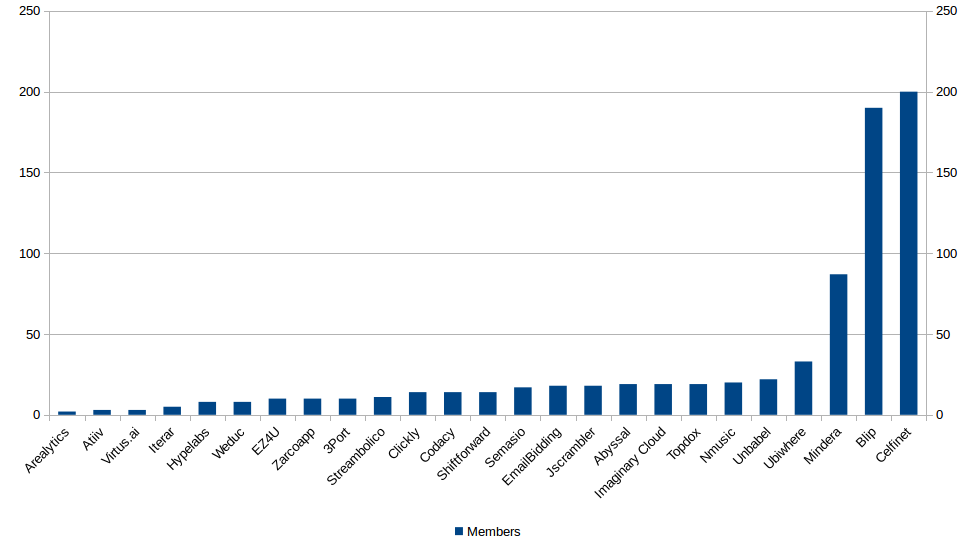
\includegraphics[width=1\linewidth]{companymembers}
        \caption{Studied companies size}
        \label{fig:companymembers}
      \end{figure}

      \subsection{Data Processing \& Pattern Extraction}
      After conducting the interviews, the next task was to analyze and process the collected information.\\
      Fig. \ref{fig:concepts} shows how we merged some of the identified techniques into larger groups that would represent patterns. The full grouping can be found in \ref{anex:pat:group}.\\
      \begin{figure}
        \centering
        \includegraphics[width=0.4\linewidth]{concepts_partial}
        \caption{Identified concepts and subsequent refining}
        \label{fig:concepts}
      \end{figure}
      As this was being done, it became clear that, because of the size of the sample (25 companies), this study would not be statistically significant. Nevetheless we found that the information we gathered had value and would be able to provide future studies with usefull pointers on how to approach the problem.\\
       Due to the fact that some practices were rare, we had to group them into categories in order to have a representative value inside the sample, e.g. some companies would run integration tests on their CI tool while others would only run unitary tests; both would, nevertheless, run tests. \\
      Using this groupings, we were able to identify a set of problems that companies were solving using different approaches. We were able, as a result, to extract in total 13 patterns each representing a problem and providing a set of solutions that took into consideration the context of the company. The final list of practices and frequencies can be found in \ref{anex:pat:freq}.
      This set of patterns can be found in chapter \ref{chap:patterns}

     \subsection{Patterns}
      Throughout the interviews we noted several tendencies. \\
      The first was the widespread use of Cloud computing with 76\% of the interviewed companies using it. Then there was the dominance of Git as the version control system with 80\% of the interviewees using it as their version control system. Chat and direct communication were also the main ways chose by companies to communicate (100\%). \\
      Being able to measure some of the key business metrics like the health of the system is also a concern for most companies with almost 70\% of them having some sort of system to do so. \\
      Having a way to replicate environments was also a major trend among companies with 60\% of companies already adopting one way to do so. \\
      The following table(tab. \ref{table:categories}) enumerates the categories of problems identified with the percentage of interviewed companies that were handling that problem. These problems will be further developed in chapter \ref{chap:patterns}

      \begin{table}[h!]
        \begin{center}
            \begin{tabular}{| p{0.5\linewidth} | p{0.5\linewidth} |}
            \hline
            \textbf{Categories} & \textbf{\% of companies that solved the problem} \\ \hline
                  Version Control                       & 100\% \\ \hline
                  Communication                         & 100\% \\ \hline
                  Cloud                                 & 84\%  \\ \hline
                  Auditability                          & 68\%  \\ \hline
                  Continuous Integration                & 64\%  \\ \hline
                  Error Handling                        & 60\%  \\ \hline
                  Reproducible Environments             & 60\%  \\ \hline
                  Scalling                              & 48\%  \\ \hline
                  Code Review                           & 44\%  \\ \hline
                  New Computing Instances Deployment    & 44\%  \\ \hline
                  Error Alerting                        & 36\%  \\ \hline
                  Job Scheduling                        & 12\%  \\ \hline
            \end{tabular}
        \end{center}
        \caption{Categories frequency}
        \label{table:categories}
      \end{table}